\chapter{Image Reconstruction}
\label{ch:imaging}
In the preceding chapter, a comprehensive analysis of the radar stability and antenna gain measurements,
were conducted to understand the factors influencing system performance over time.
Valuable insights into the temporal characteristics of the radar system were gained through this investigation,
serving as the foundation for subsequent imaging experiments.

In this chapter, the focus shifts to radar imaging.
Building upon the insights garnered from stability analysis and antenna gain measurements,
three distinct imaging algorithms are implemented and evaluated using the PyTorch framework.
These algorithms include an FFT-based approach, a Backprojection method, and a hybrid algorithm combining elements of both.

PyTorch is introduced in \cref{app:pytorch} as a versatile tool for implementing radar processing algorithms.
Following this, the implementation and evaluation of three distinct imaging algorithms is described:
\cref{sec:fft_imaging} focuses on FFT-Based Imaging, where we explore the offline calibration,
assess \emph{Direction of Arrival} (DOA) accuracy,
and present test images. In Section 3, we shift our attention to Backprojection Imaging,
examining DOA accuracy and showcasing test images. Section 4 introduces the Hybrid Approach,
where we evaluate DOA accuracy and present test images.
Finally, Section 5 provides a comprehensive summary,
comparing and analyzing the performance of the three algorithms to provide insights into their respective strengths and limitations.

\section{PyTorch}
\label{app:pytorch}
The algorithms implemented in this chapter are presented in the PyTorch framework.
As a machine learning framework, it provides accelerated tensor processing.
Tensors, ie.\ rectangular multidimensional arrays are a perfect fit to
describe the signals sent by the sensor and the subsequent signal processing.

Given that a significant portion of the operations in the imaging algorithms are parallelizable,
considerable performance gains can be achieved with the built-in parallel processing of tensor operations in PyTorch.
While parallel processing on a CPU already improves runtimes substantially,
even better performance can be attained with GPU-enabled parallel processing,
which is currently available using the CUDA-API on NVIDIA GPUs.

To aid in understanding any code listings referenced in this chapter,
a brief tutorial is included in \cref{app:pytorch_tutorial}
that discusses some key parts of PyTorch's syntax for tensor processing.

\section{FFT-Based Imaging}
\label{sec:fft_imaging}
The first imaging algorithm to be implemented is based on the FFT.
A detailed description of the algorithm can be found in \cref{sec:dft_imaging_theory},
but the following is an abrigded summary to reiterate the key principles.

The range is estimated by computing the FFT spectrum of each time signal;
due to the FMCW principle, the frequency of the received signal is directly related to its range.
Then, making the assumption of planar incident waves
as well as having calibrated the array to achieve coherence between channels,
the angle of arrival can be estimated using FFTs over the ULA subset of the sensor's virtual antenna array.
The resolution can be increased by zero-padding the signal before applying the FFT.
An example implementation in PyTorch is shown in code listing \ref{lst:fft_img}.

Here, the function \verb|calc_image| returns a 3D-image of dimension $N_{range} \times N_{azimuth} \times N_{elevation}$.
Its input consists of \verb|data|, a time data tensor of dimension $M \times K$,
the calibration weights \verb|weights| of dimension $K$, and \verb|settings|, a dictionary of settings.
\verb|settings| is expected to contain the input and output dimensions,
the indices of the ULA subset of the virtual array with gaps indicated by $-1$,
as well as the window functions to be used in each FFT.

\subsection{Direction of Arrival Accuracy}
\label{sec:fft_doa}
This section aims to illustrate the theoretical capabilities of FFT-based DoA-estimation on the iMCR.
The directivity in azimuth and elevation is simulated for multiple distances to illustrate the impact of near-field conditions.
\\

For this, the input time signal is an ideal point source (see eqn.\ \ref{eq:ideal_scatterer}),
located at $(R,\theta=0,\phi=0)$
assuming a constant channel gain of $\underline C_k(r,0,0)=1 \,\forall r,k$:
\begin{align}
    \underline y_k[m] =  e^{-j\dot \omega \tau_k m T_s}    ,\,k\in[0,K-1],m\in[0,M-1]
\end{align}
The time of flight $\tau_k$ is computed using the physical measurements of the array.
\\
The image is computed for multiple distances at resolution
$N_{range} = 1024, N_{azimuth} = 2048$ and $N_{elevation} = 8$.
and evaluated at the range and evaluation bin of the scatterer.
The resulting peaks in azimuth are shown in \cref{fig:fft_azm_peak}.
\begin{figure}[h]
    \centering
    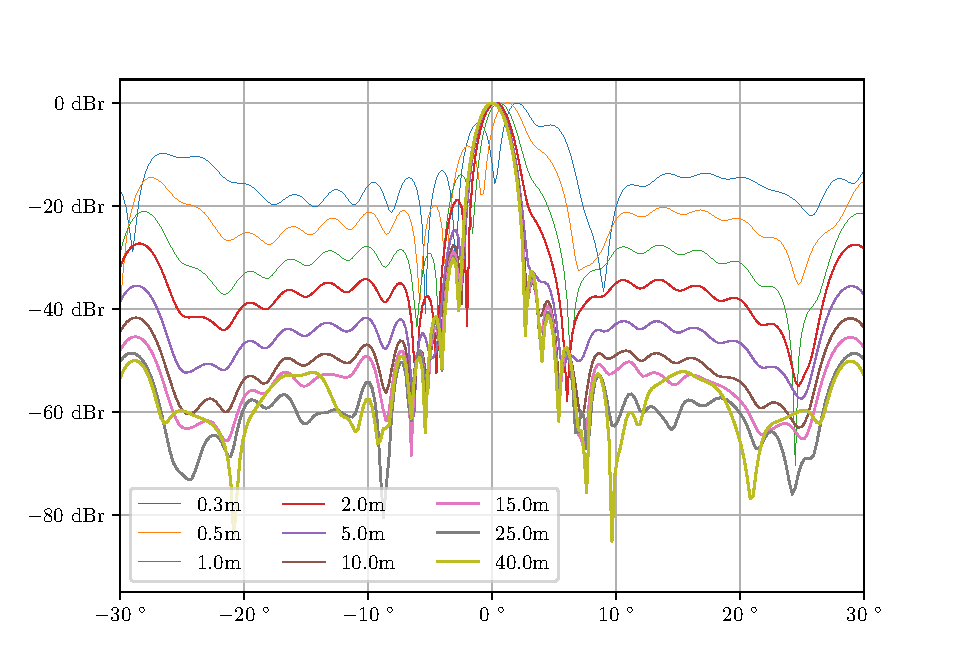
\includegraphics[width=\textwidth]{../figures/fft_azm_peak.pdf}
    \caption{iMCR FFT direction of arrival estimation: theoretical accuracy in azimuth for an ideal point scatterer at different ranges}
    \label{fig:fft_azm_peak}
\end{figure}

The Fraunhofer distance of the array can be computed from the wavelength $\lambda_0=$ \SIlist{3.944}{\mm}
and the virtual array's azimuth aperture $D_{azm} = 86 \frac{\lambda_0}{2}=$ \SI{16.96}{\cm}:
\begin{align}
    d_f  = \frac{2D_{azm}^2}{\lambda_0}
    = \SI{14.59}{\m}
\end{align}
It can be seen that for targets closer than $d_f$, the peak deteriorates in multiple ways.
The location of the peak moves to higher angles than the actual location of $\theta =$ \SI{0}{\degree}.
For targets at \SI{30}{\cm}, the peak has moved to $\theta =$ \SI{2.02}{\degree}.

In near-field conditions, the side lobe levels increase until their minimum only around \SI{20}{\dB} below the peak,
whereas in the far field, the minimum is \SI{60}{\dB} below the peak.

In far-field conditions, the main peak at $\theta =$ \SI{0}{\degree}
is clearly separated from its sidelobes by pronounced local minima.
The minimum to the right of the main peak starts to disappear below $d_f$,
and the peak to the right starts to merge with the main peak the closer the target gets.
The far-field half-power and quarter-power beamwidths are approximately
$\theta_{\SI{3}{\dB}}=$ \SI{1.9}{\degree} and $\theta_{\SI{6}{\dB}}=$ \SI{2.6}{\degree}, respectively. \\
% \begin{figure}[h]
%     \centering
%     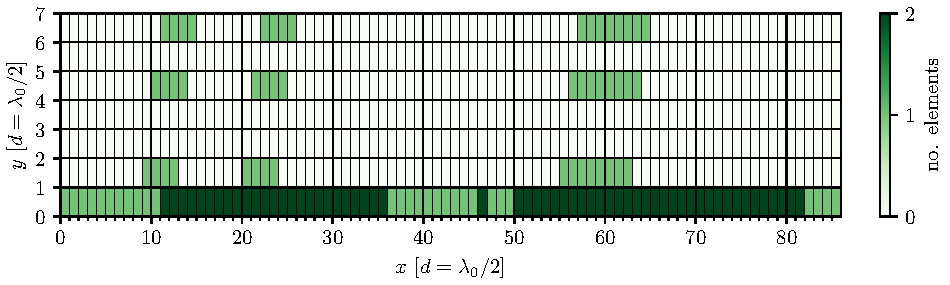
\includegraphics[width=\textwidth]{../figures/virt_array.pdf}
%     \caption{iMCR virtual antenna array occupancy}
%     \label{fig:virt_array}
% \end{figure}

For direction of arrival estimation in azimuth, the 86-channel ULA subset of the array is well applicable to an FFT-based approach,
even with its reduced performance in near-field conditions.
Yet in elevation, such a ULA subset does not exist, as the array is sparse in elevation,
both horizontally and vertically (c.f.\ \ref{fig:imcr_virt_array}):
in most collums, only one virtaul antenna is present.

To still use the FFT, a possible approach would be ``backfilling'' the array with zeros
to obtain a complete uniformly spaced rectangular virtual array.
The FFT is then computed over the collumns (c.f.\ \ref{fig:imcr_virt_array}) of the resulting URA,
each yielding a spectrum that is related to the direction of arrival in elevation.

A disadvantage of this approach is that it can cause substantial spectral leakage.
Our backfilled array $b[k] $ is mathematically equivalent
to applying a binary window function $w[k]$ to the ideal rectangular array $a[k]$:
\begin{align*}
    b[k]                   & =  w[k] \cdot  a[k]             \\
    \text{e.g.}\;  b[0..7] & = [b_0, b_1, 0,0,b_2,0,b_3,0 ], \\
    w[0..7]                & = [1,  1,0,0,1,0,1,0 ],         \\
    \text{and}\; a[0..7]   & = [a_0,a_1,a_2,\dots,a_7]
\end{align*}

However, this window function causes additional peaks to appear in the spectrum,
since multiplication in the time domain is equivalent to convolution in the frequency domain:
\begin{align*}
    \mathcal{F}\{b[k]\}[n] & = \mathcal{F}\{w[k] \cdot  a[k]   \}[n] \\
                           & = W[n] * A[n]
\end{align*}
In case of the example given above,
\begin{align*}
    |W[0..7]| = [4.00,\ 0.77,\ 1.41,\ 1.85,\ 2.00,\ 1.85,\ 1.41,\ 0.77]
\end{align*}

It would be possible to reduce the spectral leakage with deconvoltion algorithms.
To show the starting point for these algorithms,
the unadulterated spectral peak for targets at multiple distances is shown in \cref{fig:fft_elv_peak}.

\begin{figure}[h]
    \centering
    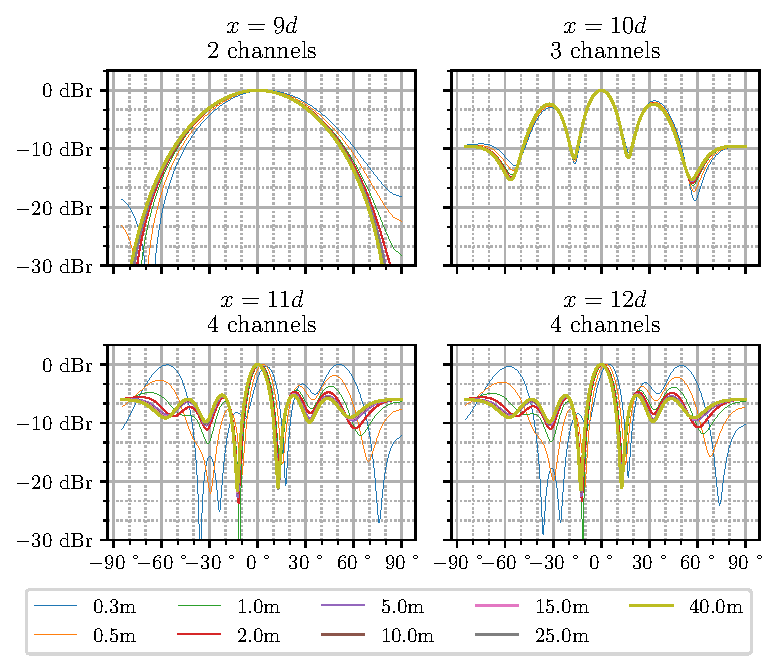
\includegraphics[width=0.8\textwidth]{../figures/fft_elv_peak.pdf}
    \caption{iMCR FFT-based direction of arrival: theoretical accuracy in elevation for an ideal point scatterer at different ranges and different array subsets}
    \label{fig:fft_elv_peak}
\end{figure}

It can be seen that the half-power beamwidth improves the more channels are included in the sub-array:
for two, three and four active channels, we approximately get
$\phi_{\SI{3}{\dB}}=$ \SIlist{60;14;12}{\degree}, respectively.

As the peak narrows, the spectrum contains more and more sidelobes.
For sub-arrays that include three channels, the side peaks are the strongest,
barely \SI{3}{\dB} less than the main peak. \\

The Fraunhofer distance of the array in elevation can be computed from the wavelength $\lambda_0=$ \SIlist{3.944}{\mm}
and the virtual array's maximal elevation aperture $D_{elv} = 7 \frac{\lambda_0}{2}=$ \SI{1.38}{\cm}:
\begin{align}
    d_f  = \frac{2D_{elv}^2}{\lambda_0}
    = \SI{9.66}{\cm}
\end{align}
The Frauenhofer distance in elevation is smaller than in azimuth by an order of magnitude.
Thus, all distances considered lie in the far-field,
and the shape of the peak should not change a lot over distance.

While this holds true for the two-- and three-channel case, if four channels are considered,
the shape does change with distance.

On the one hand, the location of the main peak moves to higher angles if the range is decreased.
On the other hand, the first two sidelobes decrease in amplitude,
while the third ones move towards $\phi=$ \SI{0}{\degree} and increase in amplitude.

\subsection{Offline Calibration}
To compute the angle of arrival, it is critical that the input signal be coherent in both amplitude and phase.

This is done by deviding each channel's range spectrum $Y_k(\Omega)$ by its corresponding estimate channel gain $\hat C_k e^{j\hat \varphi_k}$.
As well as aligning the phases correctly, this also equalizes the channel gains.
Note that this approach does not take the channel gain pattern into account, but only its static amplitude,
since the same channel gain estimate is used for all directions. \\

\newpage
\subsection{Test Image}
\label{sec:fft_result}
To give an indication how well the theoretical capabilities of the FFT-based approach translate into real world applications,
a test scene was recorded. The sensor is placed facing the front of a building with circular walls, and
a reflector is placed between them, slightly off-center at a distance of approximately \SI{6}{\m}.

The target 2D image spans a $24 \times$\SI{15}{\m} area in the horizontal plane,
with square pixels of edge length \SI{10}{\cm},
and the sensor located on one of the image's long sides, namely $[x,y] = [0,0]$.

It is constructed by first calculating the polar-coordinate FFT image at a resolution of $N_{range}\times N_{azimuth} = 2048 \times 512$.
The image can then be extracted from by selecting the range- and azimuth bins $m$ and $k$ that correspond to each pixel $[x,y]$:
\begin{align}
    m & = \left\lfloor N_{range} \frac{\sqrt{x^2 + y^2} }{R_{max}} \right\rfloor                              \\
    k & = \left\lfloor \frac{N_{azimuth}}{2} \left(\sin\arctan\left(\frac{y}{x}\right)+1\right) \right\rfloor
\end{align}

\cref{fig:fft_testimg} shows the resulting image with and without calibration.
\begin{figure}
    \centering
    \begin{subfigure}{0.8\textwidth}
        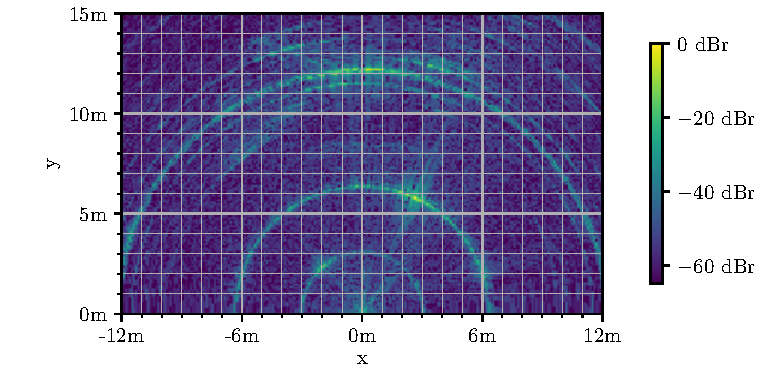
\includegraphics[width=\textwidth]{../figures/testimg_uncalibrated_fft.pdf}
        \subcaption{uncalibrated}
    \end{subfigure}
    \begin{subfigure}{0.8\textwidth}
        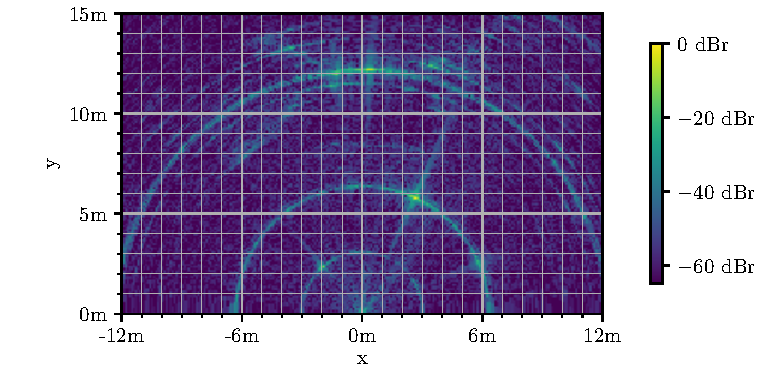
\includegraphics[width=\textwidth]{../figures/testimg_calibrated_fft.pdf}
        \subcaption{calibrated}
    \end{subfigure}
    \caption{FFT-based image generated from real data}
    \label{fig:fft_testimg}
\end{figure}
It can be seen that increases output SNR, which results in a higher contrast image.
Also, the azimuth response improves, decreasing the width of the peak caused by the reflector.
Furthermore, in the calibrated image, the outline of the tower is easier to make out.
Altogether, the image still contains too many artifacts in azimuth:
each peak of the image coincides with a semi-circle centered on the sensor.
We have shown that this behaviour is expected in \cref{sec:fft_doa}:
the theoretically achievable main lobe without windowing is about \SI{40}{\dB} higher than the others.
To improve image clarity, a decrease in dynamic range through thresholding may be required.

\section{Backprojection Imaging}

The second imaging algorithm to be implemented is backprojection.
A detailed description of the algorithm can be found in \cref{sec:bp_imaging_theory},
but the gist of it is the following:

Backprojection works by computing the correlation between the incoming time data
and the signal of an isotropic scatterer (see \cref{eq:ideal_scatterer})
at an arbitrary set of locations.
The ideal signal for the isotropic scatterer at a given location $\vec r$
is computed using the measured complex channel gains at that location $\underline{\hat C}_k(\vec r)$:
\begin{align*}
    s_k[m] = \underline{\hat C}_k(\vec r) e^{-j\dot\omega\tau_k(\vec r)mT_s}
\end{align*}
At this point, an intensity normalization in range
could also be implemented simply multiplying the ideal signal with $r^2$.
The same is acchievable in cross-range by inverting the amplitude of the channel gains.

Since the channel gains are assumed to be static,
the ideal signals can be pre-computed for generating images for at multiple points in the long-time dimension.
An example implementation in PyTorch is shown in code listing \ref{lst:bp_img}.
\\

A major limitation implementations with pre-calculated weights is its scalability.
Pre-calculating the weights, while allowing for decent opportunites in decreasing the runtime through parallel processing,
quickly use a prohibitive amount of memory.

If there are $Z$ individual locations, $M$ sample points in time and $K$ channels, then $M \cdot K \cdot Z$ weights need to be computed.
For example, the weights for a uniformly spaced image with a rather low resolution of  $Z = 100 \cdot 10 \cdot 100 =$ \SI{100}{kilovoxels},
at $K=192$ and $M=1022$, stored as complex numbers consisting of two \SI{64}{bit} floating point numbers, would require
\begin{align*}
      & M \cdot K \cdot Z \cdot 2 \cdot \SI{64}{\bit} \\
    = & 1022 \cdot 192 \cdot 10^5 \cdot \SI{16}{byte} \\
    = & \SI{3.14e12}{byte} = \SI{3.14}{\tera\byte}
\end{align*}
of memory.
With the projections of Moore's law \cite{mooreslaw},
this amount of memory should be available in consumer-level computers by the year 2050.
Until then, the memory requirements have to be reduced by re-computing the weights
and applying them to the input data along an arbitrary dimension.
For example, recomputing them for every of the sampled time points would reduce
the memory requirements by a factor of 1022 to a more manageable size of around \SI{3}{\giga\byte}.

\begin{figure}[h]
    \centering
    \begin{subfigure}[t]{\textwidth}
        \centering
        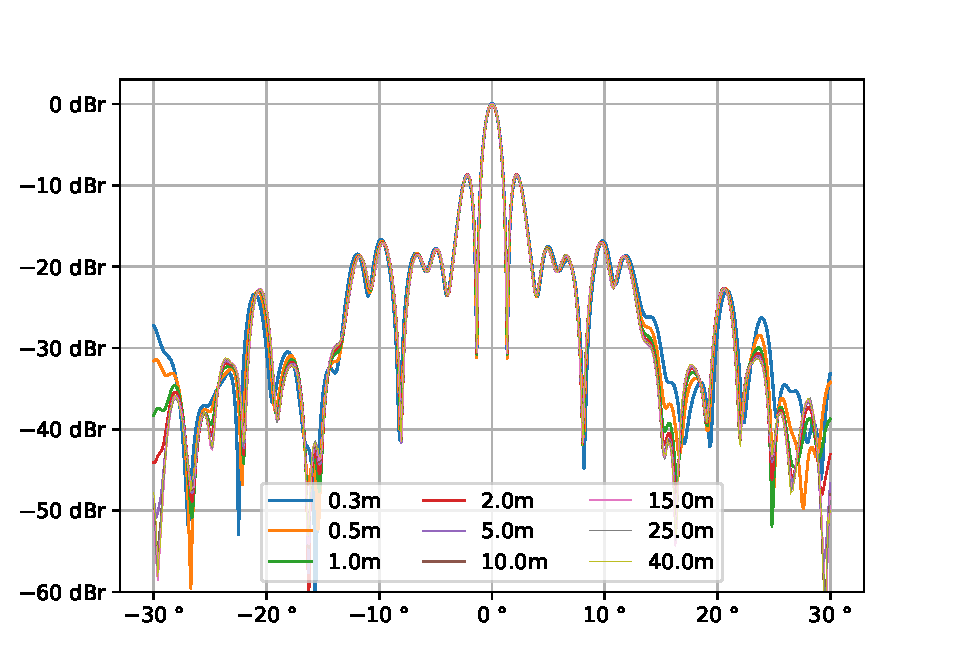
\includegraphics[width=\textwidth]{../figures/bp_azm_peak.pdf}
        \subcaption{azimuth}
        \label{fig:bp_azm_peak}
    \end{subfigure}

    \begin{subfigure}[position]{\textwidth}
        \centering
        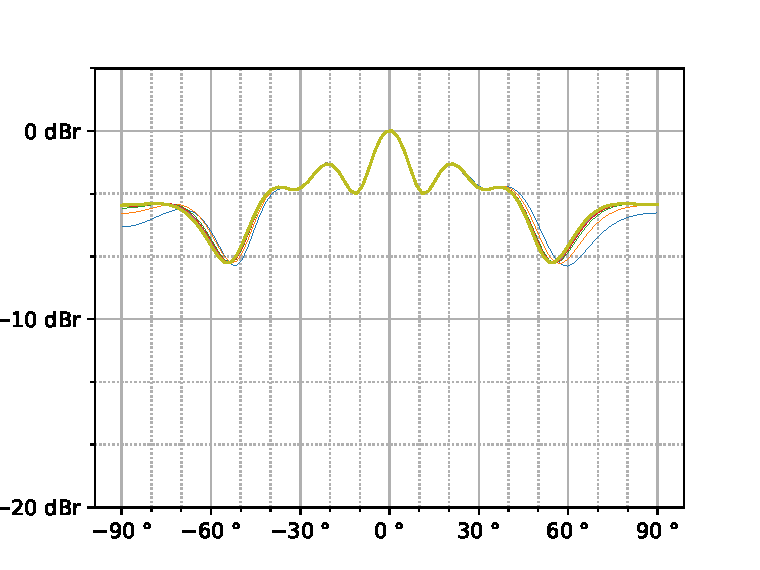
\includegraphics[width=0.8\textwidth]{../figures/bp_elv_peak.pdf}
        \subcaption{elevation}
        \label{fig:bp_elv_peak}
    \end{subfigure}

    \caption{iMCR backprojection direction of arrival estimation: theoretical accuracy for an ideal point scatterer at different ranges}
\end{figure}
\subsection{Direction of Arrival Accuracy}

To better understand the DoA-estimation capabilities of the algorithm,
the azimuth and elevation response is simulated for multiple distances to illustrate the impact of near-field conditions.
The same input signal as in \cref{sec:fft_doa} is used.
\\

The image is computed for multiple distances at resolution
$N_{range} = 1$, ${N_{azimuth} = 512}$ and $N_{elevation} = 1$.
Naturally, the range of the image is set to the range of the ideal target each time.
The resulting peaks in azimuth and elevation are shown in figures \ref{fig:bp_azm_peak} and \ref{fig:bp_elv_peak}, respectively.


In both azimuth and elevation, it can be seen that the peak no longer deteriorates in what were near-field conditions for the FFT-based approach.
The peak and most side lobes remain virtually identical across all considered ranges.
Essentially, the backprojection algorithm has brought Frauenhofer distance closer in range,
because the array is re-focused for every inspected point.
In azimuth, the level of the sidelobes stabilizes at around \SIrange{30}{40}{\dB} below the peak,
whereas in elevation, the sidelobe level is merely \SIrange{3}{6}{\dB} below the peak.

The azimuth half-power beamwidth is approximately $\theta_{\SI{3}{\dB}}=$ \SI{1.6}{\degree} and
the azimuth quarter-power beamwidth approximately $\theta_{\SI{6}{\dB}}=$ \SI{2.4}{\degree}.
In elevation, the half-power beamwidth is approximately $\phi_{\SI{3}{\dB}}=$ \SI{20}{\degree} and
the quarter-power beamwidth approximately $\phi_{\SI{6}{\dB}}=$ \SI{100}{\degree}.


A possible way to increase directivity in elevation is to increase the elevation channels' impacts by applying higher weights to them.
Since 13 of 16 Rx-antennas are located at the same height, their impact on the elevation response is disproportionately high.


\newpage
\subsection{Test Image}
The theoretical capabilities of the backprojection algorithm are again tested for real world applications,
using the same scene as in \cref{sec:fft_result}.

Once again, the target 2D image spans a $24 \times$\SI{15}{\m} area in the horizontal plane,
with square pixels of edge length \SI{10}{\cm},
and the sensor located on one of the image's long sides, namely $[x,y] = [0,0]$m.
Unlike the FFT-based approach,
the backprojection algorithm allows for an arbitrary set of sample points,
so no further transformations are required to obtain an image with square pixels.\\
\begin{figure}[t]
    \centering
    \begin{subfigure}{0.8\textwidth}
        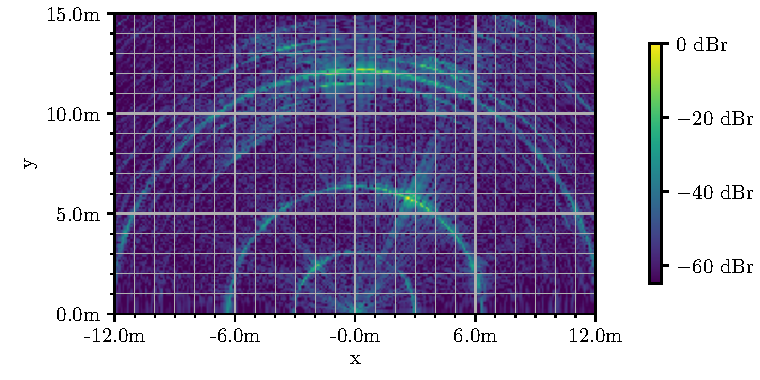
\includegraphics[width=\textwidth]{../figures/testimg_uncalibrated_bp.pdf}
        \subcaption{uncalibrated}
    \end{subfigure}
    \begin{subfigure}{0.8\textwidth}
        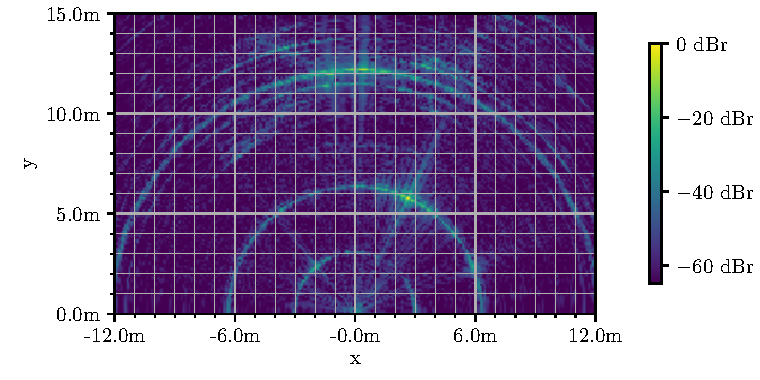
\includegraphics[width=\textwidth]{../figures/testimg_calibrated_bp.pdf}
        \subcaption{calibrated}
    \end{subfigure}
    \caption{Backprojection image generated from real data}
    \label{fig:bp_testimg}
\end{figure}
In \cref{fig:bp_testimg}, the resulting images obtained with and without calibration are compared.
Calibration demonstrates several notable effects:
Calibration leads to an enhanced SNR and a reduction in the width of azimuth peaks.
Additionally, the influence of antenna gain patterns becomes apparent,
causing attenuation in off-center regions and for longer distances.
As predicted in the previous section,
the direction of arrival estimation is not perfect, even for ideally calibrated data.
Each peak is accompanied by a circular artifact at the same range, concentric to the sensor.

Compared to FFT imaging, the noise attenuation appears to have improved for both images.
This expected, since the FFT-approach only uses 86 out of the 192 available channels,
while backprojection uses all of them.
This should lead to up to double the noise attenuation,
as the following brief detour into estimation theory will explain.

Doubling the number of samples in the presence of any additive zero-mean noise
can lead to a halving of the noise variance due to the properties of the sample mean estimator
and the central limit theorem.
The sample mean estimator is given by:

\begin{align}
    \hat{\mu} = \frac{1}{N} \sum_{i=1}^{N} x_i
\end{align}

where $ x_i $ are the individual samples and $ N $ is the number of samples.
The variance of the sample mean estimator is given by:

\begin{align}
    \text{Var}(\hat{\mu}) = \frac{\sigma^2}{N}
\end{align}

where $ \sigma^2 $ is the variance of the noise.

As the number of samples $N$ increases,
the variance of the sample mean estimator decreases proportionally to $\frac{1}{N}$.
Hence, doubling the number of samples effectively halves the noise variance,
resulting in a more accurate estimate of the true value.

\newpage
\section{Hybrid Approach}
\label{sec:hybrid_imaging}
Compared to the FFT-based approach, the backprojection algorithm is a lot more computationally intensive,
taking multiple orders of magnitude longer to compute a single 2D image.
The runtime of the implemented algorithm confirms the results from the complexity analysis in \cref{sec:complexity_analysis}:
while the FFT-based approach has a complexity of $\mathcal O(MK\log MK)$, the backprojection approach costs $\mathcal O(ZMK)$.

As explained in \cref{sec:bp_imaging_theory},
it is possible to replace part of the computation with an inverse FFT,
taking advantage of the increased speed and lower memory consumption of the inverse FFT-algorithm,
while sacrificing some accuracy.
An example implementation of the backprojection-FFT-hybrid algorithm can be found in \ref{lst:hybrid_img}.
Its theoretical performance is investigated in the next section. Afterwards, a test image is computed.

\subsection{Direction of Arrival Accuracy}

Due to the inherent frequency quantization of the FFT,
this hybrid approach is prone to get inaccurate estimates of the actual backprojection of a channel.
This mismatch between the actual frequency to analyse, and the closest sampled frequency in the computed FFT
can be reduced by zero-padding the input signal to increase the sample density.

To better understand how the accuracy of DOA estimation is affected by this,
the azimuth response is simulated for multiple input lenghts.
The same input signal as in \cref{sec:fft_doa} is used, only this time, a single distance is evaluated.
\cref{fig:hybrid_azm_peak} shows the result of this simulation.
\begin{figure}
    \centering
    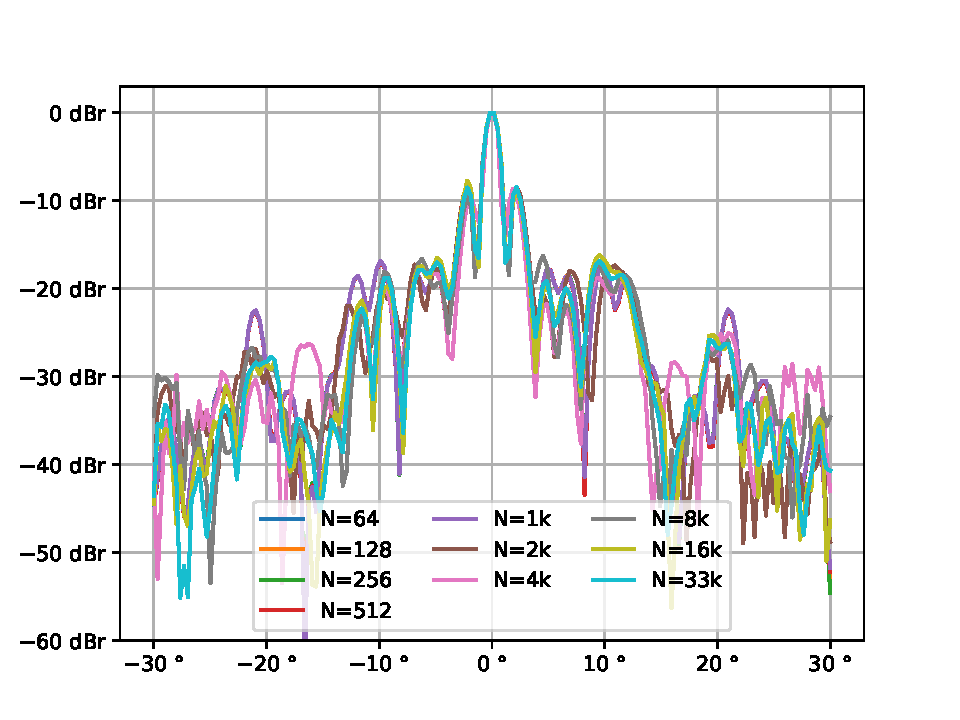
\includegraphics[width=\textwidth]{../figures/hybrid_azm_peak.pdf}
    \caption{iMCR Backprojection-FFT-Hybrid direction of arrival estimation:
        theoretical accuracy in azimuth for an ideal point scatterer at different spectral resolutions}
    \label{fig:hybrid_azm_peak}
\end{figure}

It can be seen that the main lobe and the first two side lobes stay identical in shape.
The rest of the azimuth response is more strongly affected by the spectral resolution.
However, the level of the minor lobes stays more or less unchanged,
confirming the feasibility of the hybrid approach.

\begin{figure}[b]
    \centering
    \begin{subfigure}{0.8\textwidth}
        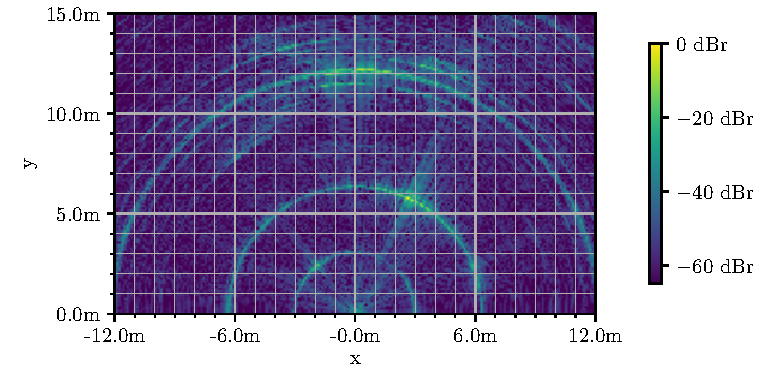
\includegraphics[width=\textwidth]{../figures/testimg_uncalibrated_hybrid.pdf}
        \subcaption{uncalibrated}
    \end{subfigure}
    \begin{subfigure}{0.8\textwidth}
        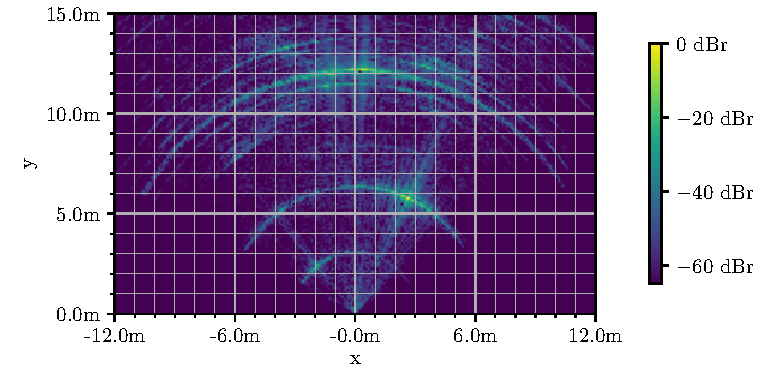
\includegraphics[width=\textwidth]{../figures/testimg_calibrated_hybrid.pdf}
        \subcaption{calibrated}
    \end{subfigure}
    \caption{Backprojection-FFT-Hybrid image generated from real data}
    \label{fig:hybrid_testimg}
\end{figure}
\subsection{Test Image}
The theoretical capabilities of the hybrid approach are put under the same test as the two previous algorithms.
Once again, the target 2D image spans a $24 \times$\SI{15}{\m} area in the horizontal plane,
with square pixels of edge length \SI{10}{\cm},
and the sensor located on one of the image's long sides, namely $[x,y] = [0,0]$m.

The resulting images looks very similar to those generated by the pure backprojection algorithm.
Calibration leads to an enhanced SNR and a reduction in the width of azimuth peaks.
Additionally, the influence of antenna gain patterns becomes apparent,
causing attenuation in off-center regions and for longer distances.
The direction of arrival estimation is not perfect, even for ideally calibrated data.
Each peak is accompanied by a circular artifact at the same range, concentric to the sensor.
The level of the circular artifact is slightly higher when compared to the pure backprojection algorithm.


\newpage
\section{Conclusion}
In this chapter, we embarked on a comprehensive exploration of radar imaging algorithms,
evaluating their performance and efficacy in extracting meaningful information from radar data.
Leveraging the insights gained from stability analysis and antenna gain measurements conducted in previous sections,
we conducted a detailed examination of FFT-based imaging, Backprojection, and a hybrid approach.
Through a systematic comparison of the resulting images and analysis of key metrics such as the azimuth and elevation peak widths,
we gained a deeper understanding of the capabilities of each algorithm.


\begin{table}[b]
    \begin{tabular}{llll}
        \toprule
        \textbf{Variable} & \textbf{FFT}              & \textbf{Backprojection} & \textbf{Hybrid}                           \\
        \midrule
        HPBW, azimuth     & \SI{1.9}{\degree}         & \SI{1.6}{\degree}       & \SI{1.6}{\degree}                         \\
        HPBW, elevation   & \SIrange{12}{60}{\degree} & \SI{20}{\degree}        & \SI{20}{\degree}                          \\
        near-field        & \SI{14.50}{\m}            & \SI{30.4}{\mm}          & \SI{30.4}{\mm}                            \\
        complexity        & $\mathcal O (MK \log MK)$ & $\mathcal O(ZM^2K)$     & $\mathcal O \left(K(Z + M\log M) \right)$ \\
        test image runtime\footnote{
            the runtime to compute the $240 \times 150$ pixel
            image.
            calculated by running the respective
            PyTorch implementation for 1000 times and taking the average.
            The time needed to transform the FFT-approach's output into cartesian coordinates was not considered.
            CPU used: 13th Gen Intel\textregistered Core\texttrademark i7-13700K
            RAM: \SI{64}{\giga\byte}
        }                 & \SI{1.4}{\ms}             & \SI{70.87}{\s}          & \SI{95.9}{\ms}                            \\
        input             & ULA or URA                & any                     & any                                       \\
        output            & spherical                 & any                     & any                                       \\
        \bottomrule
    \end{tabular}
    \caption{Comparison between the three implemented algorithms}
    \label{tab:imaging_comp}
\end{table}

A comparison of the three implemented algorithms is given in \cref{tab:imaging_comp}.
To start, the theoretically achieveable half-power beamwidths are compared.
In azimuth, the backprojection-based algorithm fair slightly better than the FFT, reaching \SI{1.6}{\degree} instead of \SI{1.9}{\degree}.
In elevation, he approach for FFT-based DOA estimation can achieve a lower HPBW (\SI{12}{\degree}) than backprojection (\SI{20}{\degree})
if an appropriate vertical sub-array is selected.
Note however that these vertical sub-arrays only consist of a maximum of four antennas,
while the backprojection based DOA estimation always uses the entire array, resulting in a higher SNR.
This effect is also seen in the SNR of the test images,
where the backprojection approaches achieve an SNR of asdf for calibrated data,
while the FFT only reaches asdf.
For backprojection, a trade-off between the SNR improvement and the elevation HPBW can be made,
where elevation channels are given greater weight in the calculation.

Another advantage of the backprojection algorithms is the reduced distortion in the near-field of the array,
by essentially re-focusing it onto every point in the target image.
One could argue that this reduces the Frauenhofer distance of the array to that of a single antenna with
$D_{ant}=$ \SI{7.6}{\mm}.

The obvious disadvantage of backprojection is its complexity and runtime.
Even for a fairly low-resolution image, it takes around \SI{70.87}{\s} per frame,
making it unfeasible for real-time applications.
The hybrid approach works substantially better, achieving \SI{95.9}{\ms} per frame,
suggesting the potential for real-time capabilities with further optimization.
The FFT-based approach remains the fastest, averaging \SI{1.4}{\ms} per frame.


In conclusion, the backprojection offers significant potential for improvements in image fidelity over the FFT-approach.
The near-field degradation of the DOA estimation is resolved and the potential SNR was increased.
It offers arbitrary flexibility in the image's shape,
a more robust DOA estimation in elevation and the application of measured antenna gains.
While pure backprojection has prohibitively high runtimes,
the hybrid approach demonstrates comparable performance to the FFT,
suggesting potential for real-time capability with some optimization.

Further research is required to understand how the algorithm's performance can be enhanced
by non-uniformly weighing the input data. In the FFT-based approach,
a regular window function could be used to enhance the shape of the peak in range and reduce its side-lobe level.
DOA-estimation could also be improved, especially in elevation,
by sacrificing some SNR gain for an enhanced HBPW by optimizing the weights for diversity.
